\begin{figure}
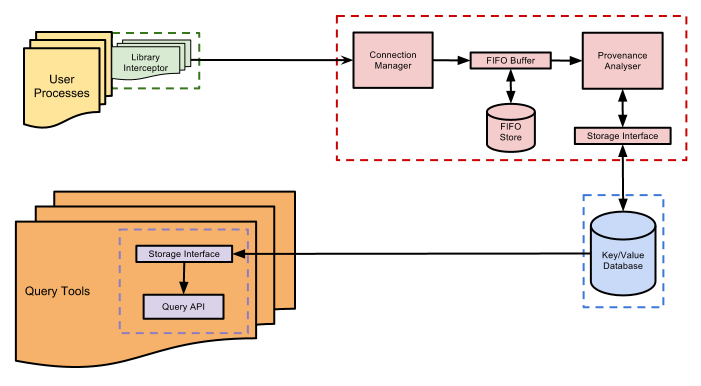
\includegraphics[width=\textwidth]{res/ProvDesign.png}
\label{fig:detdes}
\caption{Detailed design of the provenance system.}
\end{figure}

\subsubsection{Library Interceptor}
The front-end will consist of a shared library implemented in C++, which will be pre-loaded before the user application starts execution. This library will be responsible for intercepting LibC function calls by overriding the symbol table during program startup. There are tools such as PureLibc which alredy offer this functionality. However we decided to implement out own library. The reason for this decision can be found in section \ref{PurelibcJust}.

The shared library can be loaded during the start of a shell session and will track all activities that the user performs during that session. The front-end will monitor a subset of libc function calls (mainly I/O) and transmit the data to the back-end via a Unix Domain Socket (UDS). The data will be packaged using Google's Protocol buffers. The justification for using protocol buffers can be found in \ref{ProbufJust}. Each monitored I/O event will be tagged with a monotonic timestamp to indicate the actual completion of the I/O event.

\subsubsection{Connection Manager}
The back-end will consist of a thread which can accept UDS connections from the front-end clients. For each connection its corresponding UDS file descriptor will be added to the list of descriptors being monitored for data. The raw libc function data will be persisted to a log file on disk before being input into a priority queue which orders the data received based on the system's monotonic counter.

\subsubsection{Persistent Log file}
The persistent log file will provide us with the capability to analyse and debug the tool during development. It also offers the user the capability to resume a provenance trail in an event of a system or process crash. An index of checkpoint locations within the log file will also be maintained as it can provide an efficient way to rollback and resume our provenance data creation step.

\subsubsection{Provenance Analyser}
The provenance analyser thread will pull out raw provenance data from the priority queue and convert it into logical provenance objects and relations. If multiple clients send provenance data from the front-end, the back-end may not receive the data in the exact order in which the I/O events occured on the system. The priority queue will ensure that the messages are ordered by their monotonic timestamp values. A window length for processing the messages in the queue will also be enforced to compensate for packet delays.

\subsubsection{Storage Interface}
The storage interface uses a key/value database to store provenance objects. It will present a strict interface to the rest of the system allowing provenance objects to be stored and retrieved and for iteration over ranges of provenance objects. We will be implementing this using an embedded key/value database called levelDB, our justification for such can be found in Section \ref{levelDBJust}. 

\subsubsection{Key/Value Database}
The key/value store will feature five levelDB databases (tables in relational parlance). They are as follows,
\begin{itemize}
\item File and process records identified by unique provenance IDs (provID). (see section \ref{POF}).
\item I/O information for processes and files identified by I/O IDs (ioID).
\item Meta information on process execution environments identified by meta IDs (metaID).
\item An index that maps entity names to a list of provIDs.
\item An index mapping timestamp intervals to the last created provID for that interval.
\end{itemize}

%The main database will map provenance identifiers (provID) to provenance objects (see section \ref{POF}). Provenance identifiers will be unique monotonically increasing integer identifiers, they will monotonically increase to allow for a strong mapping between time and provenance identifier. The first index will map entity names to a list of all provenance entities that hold that name, ordered by increasing provID. This will allow new entries to simply be appended to the list. The second index will map timestamps to appropriate provIDs, this will be filled by inserting entries at boundaries in timestamp(e.g. every hour or every minute) containing the timestamp and the last used provID. Thus by rounding a time period to the nearest boundaries you can obtain a range of provIDs that describes the time period.

\subsubsection{Query API}
The query API will provide a wide variety of functions for retrieving provenance objects from the storage interface. It will be available initially as an importable module which any query tool can use. The strict definition of it's API has not yet been created as further investigation into the form of provenance queries needs to be made.
